\begin{center}
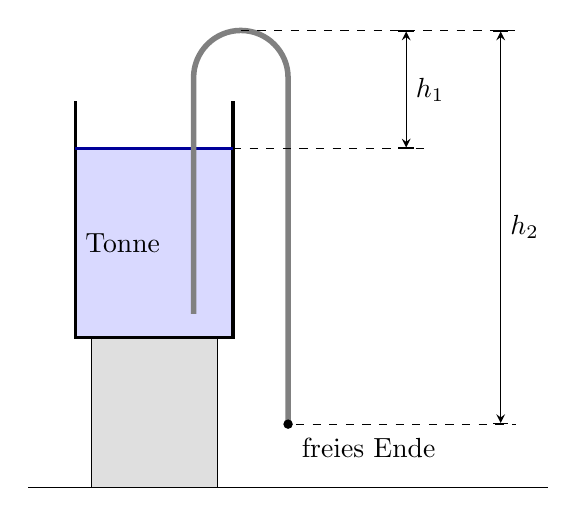
\begin{tikzpicture}[>=stealth]
 \draw (-0.6,-1.9) -- (6,-1.9);
 \fill[gray!25] (0.2,-1.9) rectangle (1.8,0);
 \draw (0.2,-1.9) rectangle (1.8,0);
 \fill[blue!15] (0,0) rectangle (2,2.4);
 \draw[very thick] (0,3) -- (0,0) -- (2,0) -- (2,3);
 \draw[blue!60!black, thick] (0,2.4) -- (2,2.4);
 \node at (0.6,1.2) {Tonne};
 \draw[line width=2pt, gray] (1.5,0.3) -- (1.5,3.3) arc (180:0:0.6) -- (2.7,-1.1);
 \fill (2.7,-1.1) circle (0.06);
 \draw[dashed] (2.1,3.9) -- (5.6,3.9);
 \draw[dashed] (2,2.4) -- (4.5,2.4);
 \draw[dashed] (2.8,-1.1) -- (5.6,-1.1);
 \draw[|<->|] (4.2,2.4) -- (4.2,3.9) node[midway, right] {$h_1$};
 \draw[|<->|] (5.4,-1.1) -- (5.4,3.9) node[midway, right] {$h_2$};
 \node[anchor=north west] at (2.75,-1.15) {freies Ende};
\end{tikzpicture}
\end{center}

Wir betrachten den höchsten Punkt des gefüllten Schlauchs. Von der Tonne her drückt dort das Wasser mit
\begin{align}
 p_1 &= p_\text{L} - \rho\,g\,h_1
\end{align}
denn an der Wasseroberfläche in der Tonne herrscht der Luftdruck $p_\text{L}$, und der höchste Punkt liegt um $h_1$ darüber. Vom freien Schlauchende her (dort herrscht ebenfalls $p_\text{L}$) drückt das Wasser mit
\begin{align}
 p_2 &= p_\text{L} - \rho\,g\,h_2
\end{align}
Solange das freie Schlauchende tiefer liegt als der Wasserspiegel in der Tonne, ist $h_2 > h_1$ und damit $p_1 > p_2$: Das Wasser wird zum freien Ende hin gedrückt und fliesst aus. Der Schlauch wirkt als Heber.

Die Tonne entleert sich deshalb, \emph{bis der Wasserspiegel in der Tonne auf der Höhe des freien Schlauchendes} liegt (dann ist $h_1 = h_2$ und das Wasser steht still), oder, wenn das freie Ende tiefer liegt als das eingetauchte Ende, \emph{bis das eingetauchte Schlauchende aus dem Wasser auftaucht} und Luft angesaugt wird. Liegt das freie Ende unter dem Tonnenboden und das andere Ende am Boden, wird die Tonne fast vollständig geleert. Der höchste Punkt des Schlauchs darf allerdings höchstens $h_1 = \hmaxF \approx \hmaxP{0}{2}$ über dem Wasserspiegel liegen (mit $p_\text{L} = \pLO$), sonst reicht der Luftdruck nicht aus, um das Wasser hochzudrücken.
